%% ----------------------------------------------------------------
%% Economic Impact of VC
%% ---------------------------------------------------------------- 

\begin{quote} 
    \centering 
        "America is the greatest engine of innovation that has ever existed, and it can't be duplicated anytime soon, because it is the product of a multitude of factors: extreme freedom of thought, an emphasis on independent thinking, a steady immigration of new minds, a risk-taking culture with no stigma attached to trying and failing, a noncorrupt bureaucracy, and financial markets and a venture capital system that are unrivaled at taking new ideas and turning them into global products"\\
    \raggedleft
        \emph{by Thomas L. Friedman}
\end{quote}

\section{Direct Effects}
    The general impact of VC is undoubtedly enormous, as was well illustrated recently by \parencite{gornall:2015}, \parencite{vc_ru_usa} and numerous other works.
    
    This effect is well quantified:
    
    \parencite{gornall:2015} find that VC-funded post-IPO companies in US:
    \begin{itemize}
        \item represent \textbf{20\%} of total market capitalisation
        \item responsible for impressive \textbf{44\%} of R\&D Expenses
        \item employ \textbf{4m people} at stable jobs, a lot of which are high-skilled
        \item generate \textbf{\$1.46 trillion} dollars of revenue in 2014
    \end{itemize}
    
    \newpage
    
    Notably, \parencite{gornall:2015} find that share of public companies VC-backing is increasing over time, as illustrated by figure \ref{fig:public_vc_backed}
    
    \begin{figure}[!htbp]
        \centering
        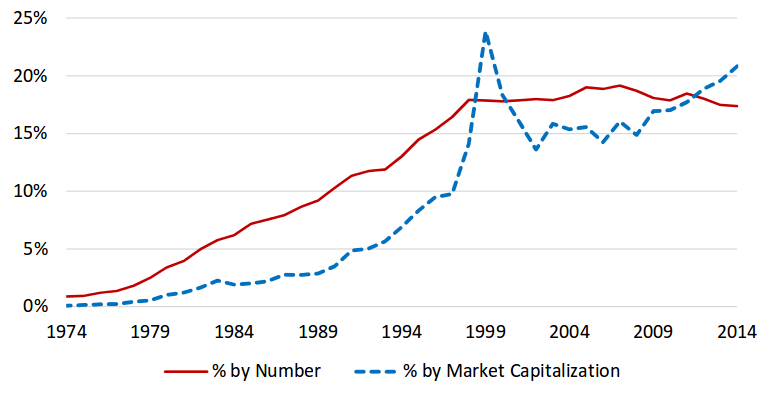
\includegraphics[scale=0.5]{public_vc_backed}
        \caption{ \textbf{Percentage of Public Companies with VC Backing by Year} \\This figure shows the percentage of independent U.S. public companies active in each year that were VC-backed. The solid red line is the percentage of VC-backed companies among those that were active in each year. The dashed blue line is the percentage on a market capitalisation weighted basis.\\Source: direct quote \parencite{gornall:2015}}
        \label{fig:public_vc_backed}
    \end{figure}
    Sharp jump in 1999-2000 is a result of doc-com bubble when markets were not functioning properly, and thus should not affect the general perception of steady growth.
    
    Same positive dynamics over time are true for the share of people employed by VC-backed ventures and increasing share of R\&D spending.
    
    Moreover, economic effect of these firms can be perceived as incremental, i.e. without VC a lot of these companies would not have had the chance to grow, as I will explain in the beginning of Chapter 03 of this thesis.


\section{Indirect Effects}
    Less quantifiable, but no less important are indirect effects of existence and innovation of these VC-backed firms.
    The most noticeable such effects are: \vspace{0.3cm}
    \begin{itemize}
        \item Participation in open-source software projects (Google, Microsoft, Red Hat, VMware are the most prominent contributors, with hundreds of smaller firms participating as well)
        \item Technological innovation \parencite{vc_ru_usa} as a result of these firms' activity benefits humanity as a whole 
        \item Disruptive technologies resulting from these startups can yield huge benefits to the society \parencite{disrupt:2015}
        \item Disintermediation \& perfect information; startups can increase information efficiency and disintermediation in many fields, to name a few\footnote{\url{https://www.crunchbase.com/}}:
        \begin{itemize}
            \item More effecient allocation of physical resources (Uber, BlaBlaCar, Airbnb etc)
            \item Financial disintermediation (Zopa, LendingClub, OnDeck Capital, Wealthfront, Betterment etc)
            \item Commerce disintermediation (eBay, Alibaba, Amazon)
            \item Perfect information about services like insurance, house rent, bank loans etc (dozens of vc-backed information aggregators)
            \item Facilitation of social interactions, professional interactions and romantic matching (Facebook, Linkedin, VC-backed dating apps) has a positive impact on the society, firms and individuals 
        \end{itemize}
        \item improved social elevator, at the time when conventional social elevator is failing in US \parencite{elevator:2010}
        \begin{itemize}
            \item Equal access to information (Google, Bing, Baidu, Wikipedia and other similar services allow \textbf{free} and \textbf{unrestricted} access to the whole enormity of human knowledge via a phone connected Internet, regardless of country or social status)
            \item Easy and often free access to education (Funding To VC-Backed Education Technology Startups Grew 503\% from 2010 to 2015 \parencite{edtech:2015} )
            \item Disrupting traditional behemoths \& oligopolies redistributes capital to startup founders and employees with equity stakes who may come from any social background
        \end{itemize}
    \end{itemize}
    
    
%% --------------------------------------------------------
%% Value-Added for VC-backed firms
%% --------------------------------------------------------

%%%%%%%%%%%%%%%%%%%%%%%%%%%%%%%%%%%%%%%%
%%%%       NEW SECTION              %%%%
%%%%%%%%%%%%%%%%%%%%%%%%%%%%%%%%%%%%%%%%
\section{Value-Added for VC-backed firms}

\begin{quote} 
    \centering 
        "We feel that without your fund's help and guidance, we'd still be pursuing a completely wrong business model with no hope of success"\\
    \raggedleft
        \emph{by grateful co-founder}
\end{quote}

The main and most obvious value that VC brings to the table is the funding itself. Especially for early-stage companies, VC may be the only viable source of funding \parencite{darin:2011} for several reasons:
\begin{itemize}
    \item Traditional financial intermediaries would not loan funds to such company because it:
    \begin{itemize}
        \item is not yet generating revenues \& profits
        \item has no reliable benchmarks and data for credit scoring to decide on an acceptable interest rate
        \item is too risky for traditional financial intermediaries
    \end{itemize}
    \item A bank requires interest payments which could be an unreasonable burden for a startup in early stages without steady revenue generation
    \item A startup requires large financial resources to grow and expand before it can start generating profits. Most prominent examples examples include, but are not limited to:
    \begin{itemize}
        \item Spotify has 100m users after 10 years of operations and produced operating losses of \$209m in 2015, according to Reuters\footnote{\url{http://www.reuters.com/article/us-spotify-users-idUSKCN0Z61FM}}
        \item Uber having more than 8m users in 400 cities still generated net losses of around \$987.2m in 2015, according to The Information \footnote{\url{http://bit.ly/28NTjz4}}
        \item Snapchat was valued at \$20 Billion\footnote{\url{http://tcrn.ch/28NyDH1}} with more than 100m Daily Active Users\footnote{\url{https://www.snapchat.com/ads}}, yet it generates little revenue, profits are a long way away
        \item the list can be continued forward, there are dozens of startups valued at billions of dollars who are yet to show a profit according to \parencite{cnn:2015}
        \item note that these companies could potentially become profitable by now, but instead VC backing allows them to pursue aggressive expansion and growth which otherwise would not has been possible
    \end{itemize}
    
\end{itemize}

Another important aspect of VC is the "value added", "smart money", or any other name for the fact that it brings external control and expertize to the companies  which positively affects their revenues and survival rates \parencite{vc_brander}.


\section{Empirical Evidence}
    For anyone remotely familiar with VC field there is no doubt that VC firms actively participate in the life of their portfolio companies, and this common knowledge is scientifically validated by \parencite{pommet}
    
    A research of German companies by \parencite{engel:2002} suggested that firms with VC financing exhibit 170\% higher growth rates than those without a VC.
    
    Positive effects extend beyond IPO, as VC-backed firms outperform their non-VC counterparts at post-IPO life \parencite{bagley}, \parencite{florin:2003}
    
    Speaking of IPO, a difficult decision to make here is timing, and research suggests that VCs help portfolio firms choose the best timing for it in order to receive the best price \parencite{hellmann:2000}
    


\section{Problems with empirical approach}
    
    Research into how VC affects startup can be questioned. On average VCs reject 99\% of all funding submissions (according to statements from many top-tier VCs) and use their experience and expertize to choose only the best ones.
    
    Thus startups are funded by VC non-randomly, on the contrary, VCs get funded \emph{because} they show sufficient promise of becoming successful due to factors usually not captured by econometric models, to name a few:
    
    \begin{itemize}
        \item Founders' expertize and previous experience
        \item Quality of their pitch and presentation (from my experience working in VC, this is surprisingly true)
        \item Solid business plan
        \item Current popularity of the type of business a startup wants to build (e.g. mobile payments, Uber-like services, etc, go through cycles of 'hype' when a huge success of some startup (usually in US) spawns copy-cats all around the globe)
        \item Other important factors which are hard to account for in a conventional model
    \end{itemize}
    
    This may create strong endogeneity in the model due to omitted variables and reverse causality. For deeper comprehension of this problem and statistical methods that can be applied as a remedy, refer to \parencite[pp. 137 - 140]{verbeek:2008}


\section{Smart Money}
    VC can add value to startups by bringing monitoring and their unique expertize. \parencite{lerner:2004}.
    
    Often VCs require board seats as part of the deal, and for a good reason: research shows that active hands-on involvement of a fund positively affects startup success chances \parencite{vc_monitoring}.
        
    Board participation gives VCs a glimpse into startups decisions, both strategic and day-to-day. As impartial business professionals, VC managers could be much more experienced than startup innovators. This can help steer the company in the right direction, achieve monetization, avoid common problems.
    
\section{Network Effect}
    VCs actively deal with many startups, socialize at events and conferences, hire talent from various industries. As a consequence, every VC has a more or less advanced network of contacts.
    For the startup this means access to:
    \begin{enumerate}
        \item other startups, firms and suppliers for synergy or co-marketing
        \item other VCs for additional funding rounds
        \item a pool of professionals for hiring
        \item reliable and motivated financiers, lawyers, accountants and other service providers otherwise not accessible to a startup
    \end{enumerate}


\section{External Control}
    VCs bring smart money approach to external control of portfolio companies via:
    
    
    \textbf{Veto Right}\\
    Even having minor equity stake, a VC may require veto rights to prevent company from executing bad tactical \& strategic decisions brought forth by the startup's management

    \textbf{Voting Majority}\\
    Often startups find themselves in a position where the VC holds voting majority, then it is fully dependent on decisions of Venture Capitalist. However the general rule is to only intervene in negative situations.
    
    
    \textbf{KPI Provisions}\\
    A good practice is setting a list of KPI (Key Point Indicators) for the firm to achieve at some point. In case of failure, the fund may:
    \begin{itemize}
        \item receive additional voting rights
        \item withhold financing (usually during a funding round, the committed sum is only transferred in pieces conditional on achieving these KPIs)
    \end{itemize}
    

    
\section{Adverse Effects}

    VC involvement often causes conflicts of interest between startup founders and venture capitalists.
    
    
    \textbf{(1) Decision making}
    
    VC wants to control startups direction and  money expenditure.
    
    Also they wish to minimise risk while increasing payoffs. This can create friction and power struggle with the founders.
    
    A good example was portraied HBO's satirical TV show "Silicon Valley" when Raviga Capital (VC investor in Pied Piper) voted their majority for the company to build a boring (but reliable in terms of everage revenue stream) b2b-oriented "black box" for servers instead of developing an innovative consumer-oriented, potentially worth billions, online platform, as the founders wanted.
    
    This can become a serious problem for the founders, since in firms on the verge of IPOs, "VCs control votes in 57\% of deals, whereas entrepreneurs control votes in 23\% of deals. Neither has control in 20\% of the cases", according to \parencite{schoar:2011}.
    
    \textbf{(2) and (3) : Valuation \& Equity Split}
    
    VC want to leave founders with as little equity to keep them motivated at minimum valuation, while startup founders want to sell VC as little equity as possible to keep them interested at maximum valuation.
    
    Adverse effects may include:
    \begin{itemize}
        \item Startups misrepresenting facts to boost valuation
        \item VCs engaging in aggressive or unethical power struggle after funding to buy out remaining founders' equity at minimal price
    \end{itemize}
    
    \textbf{(4) Exit}
    
    In VC jargon, an 'exit' is when VC fund liquidates it's shares in the company either via acquisition by some company or an IPO. 
    
    VCs are under pressure from their investors to show consistent and timely returns on investment, therefore they pressure startup management to sell out or go to IPO early. Founders would inadvertently loose equity and control over the company, and thus always become reluctant. This again creates a conflict which is always harmful for employees and businesses.
    
    It can work reversely, for if founders want to sell the company, VCs can exercise their veto rights and prevent the sale if it feels that larger returns can be gained at a later point in time.